\documentclass[border=12pt]{standalone}
\usepackage{tikz}
\usepackage{xcolor}
\usepackage{amsmath}
\usetikzlibrary{
  positioning,
  arrows.meta,
  fit,
  backgrounds,
  calc,
  shapes.geometric,
}

% ── Colour palette ──────────────────────────────────────────────────
\definecolor{textblue}{HTML}{4A90D9}
\definecolor{voicegreen}{HTML}{27AE60}
\definecolor{imagered}{HTML}{E74C3C}
\definecolor{recurrentpurple}{HTML}{8E44AD}
\definecolor{interleaveamber}{HTML}{F39C12}
\definecolor{darkgray}{HTML}{2C3E50}
\definecolor{ditteal}{HTML}{16A085}

% ── Styles ──────────────────────────────────────────────────────────
\tikzset{
  modbox/.style={
    draw=#1, fill=#1!8, rounded corners=4pt,
    minimum width=3.2cm, minimum height=0.8cm,
    font=\footnotesize\sffamily, align=center, line width=0.8pt,
  },
  widebox/.style={
    draw=#1, fill=#1!8, rounded corners=4pt,
    minimum height=0.8cm,
    font=\footnotesize\sffamily, align=center, line width=0.8pt,
  },
  annobox/.style={
    draw=#1!60, fill=#1!5, rounded corners=2pt,
    minimum width=2.4cm, minimum height=0.55cm,
    font=\scriptsize\sffamily, align=center, line width=0.5pt, dashed,
  },
  iolabel/.style={font=\scriptsize\sffamily\itshape, text=darkgray, align=center},
  attnlabel/.style={
    font=\tiny\sffamily\bfseries, rounded corners=2pt,
    fill=#1!15, draw=#1!40, inner sep=2pt,
  },
  groupbg/.style={
    draw=#1!40, fill=#1!4, rounded corners=6pt, line width=0.6pt, dashed,
  },
  arrow/.style={-{Stealth[length=5pt, width=4pt]}, line width=0.7pt, color=darkgray},
  thickarrow/.style={-{Stealth[length=6pt, width=5pt]}, line width=1.0pt, color=#1},
  dasharrow/.style={-{Stealth[length=5pt, width=4pt]}, line width=0.7pt, color=darkgray, dashed},
  thickdasharrow/.style={-{Stealth[length=6pt, width=5pt]}, line width=1.0pt, color=#1, dashed},
  seclabel/.style={font=\footnotesize\sffamily\bfseries, text=#1},
}

\begin{document}
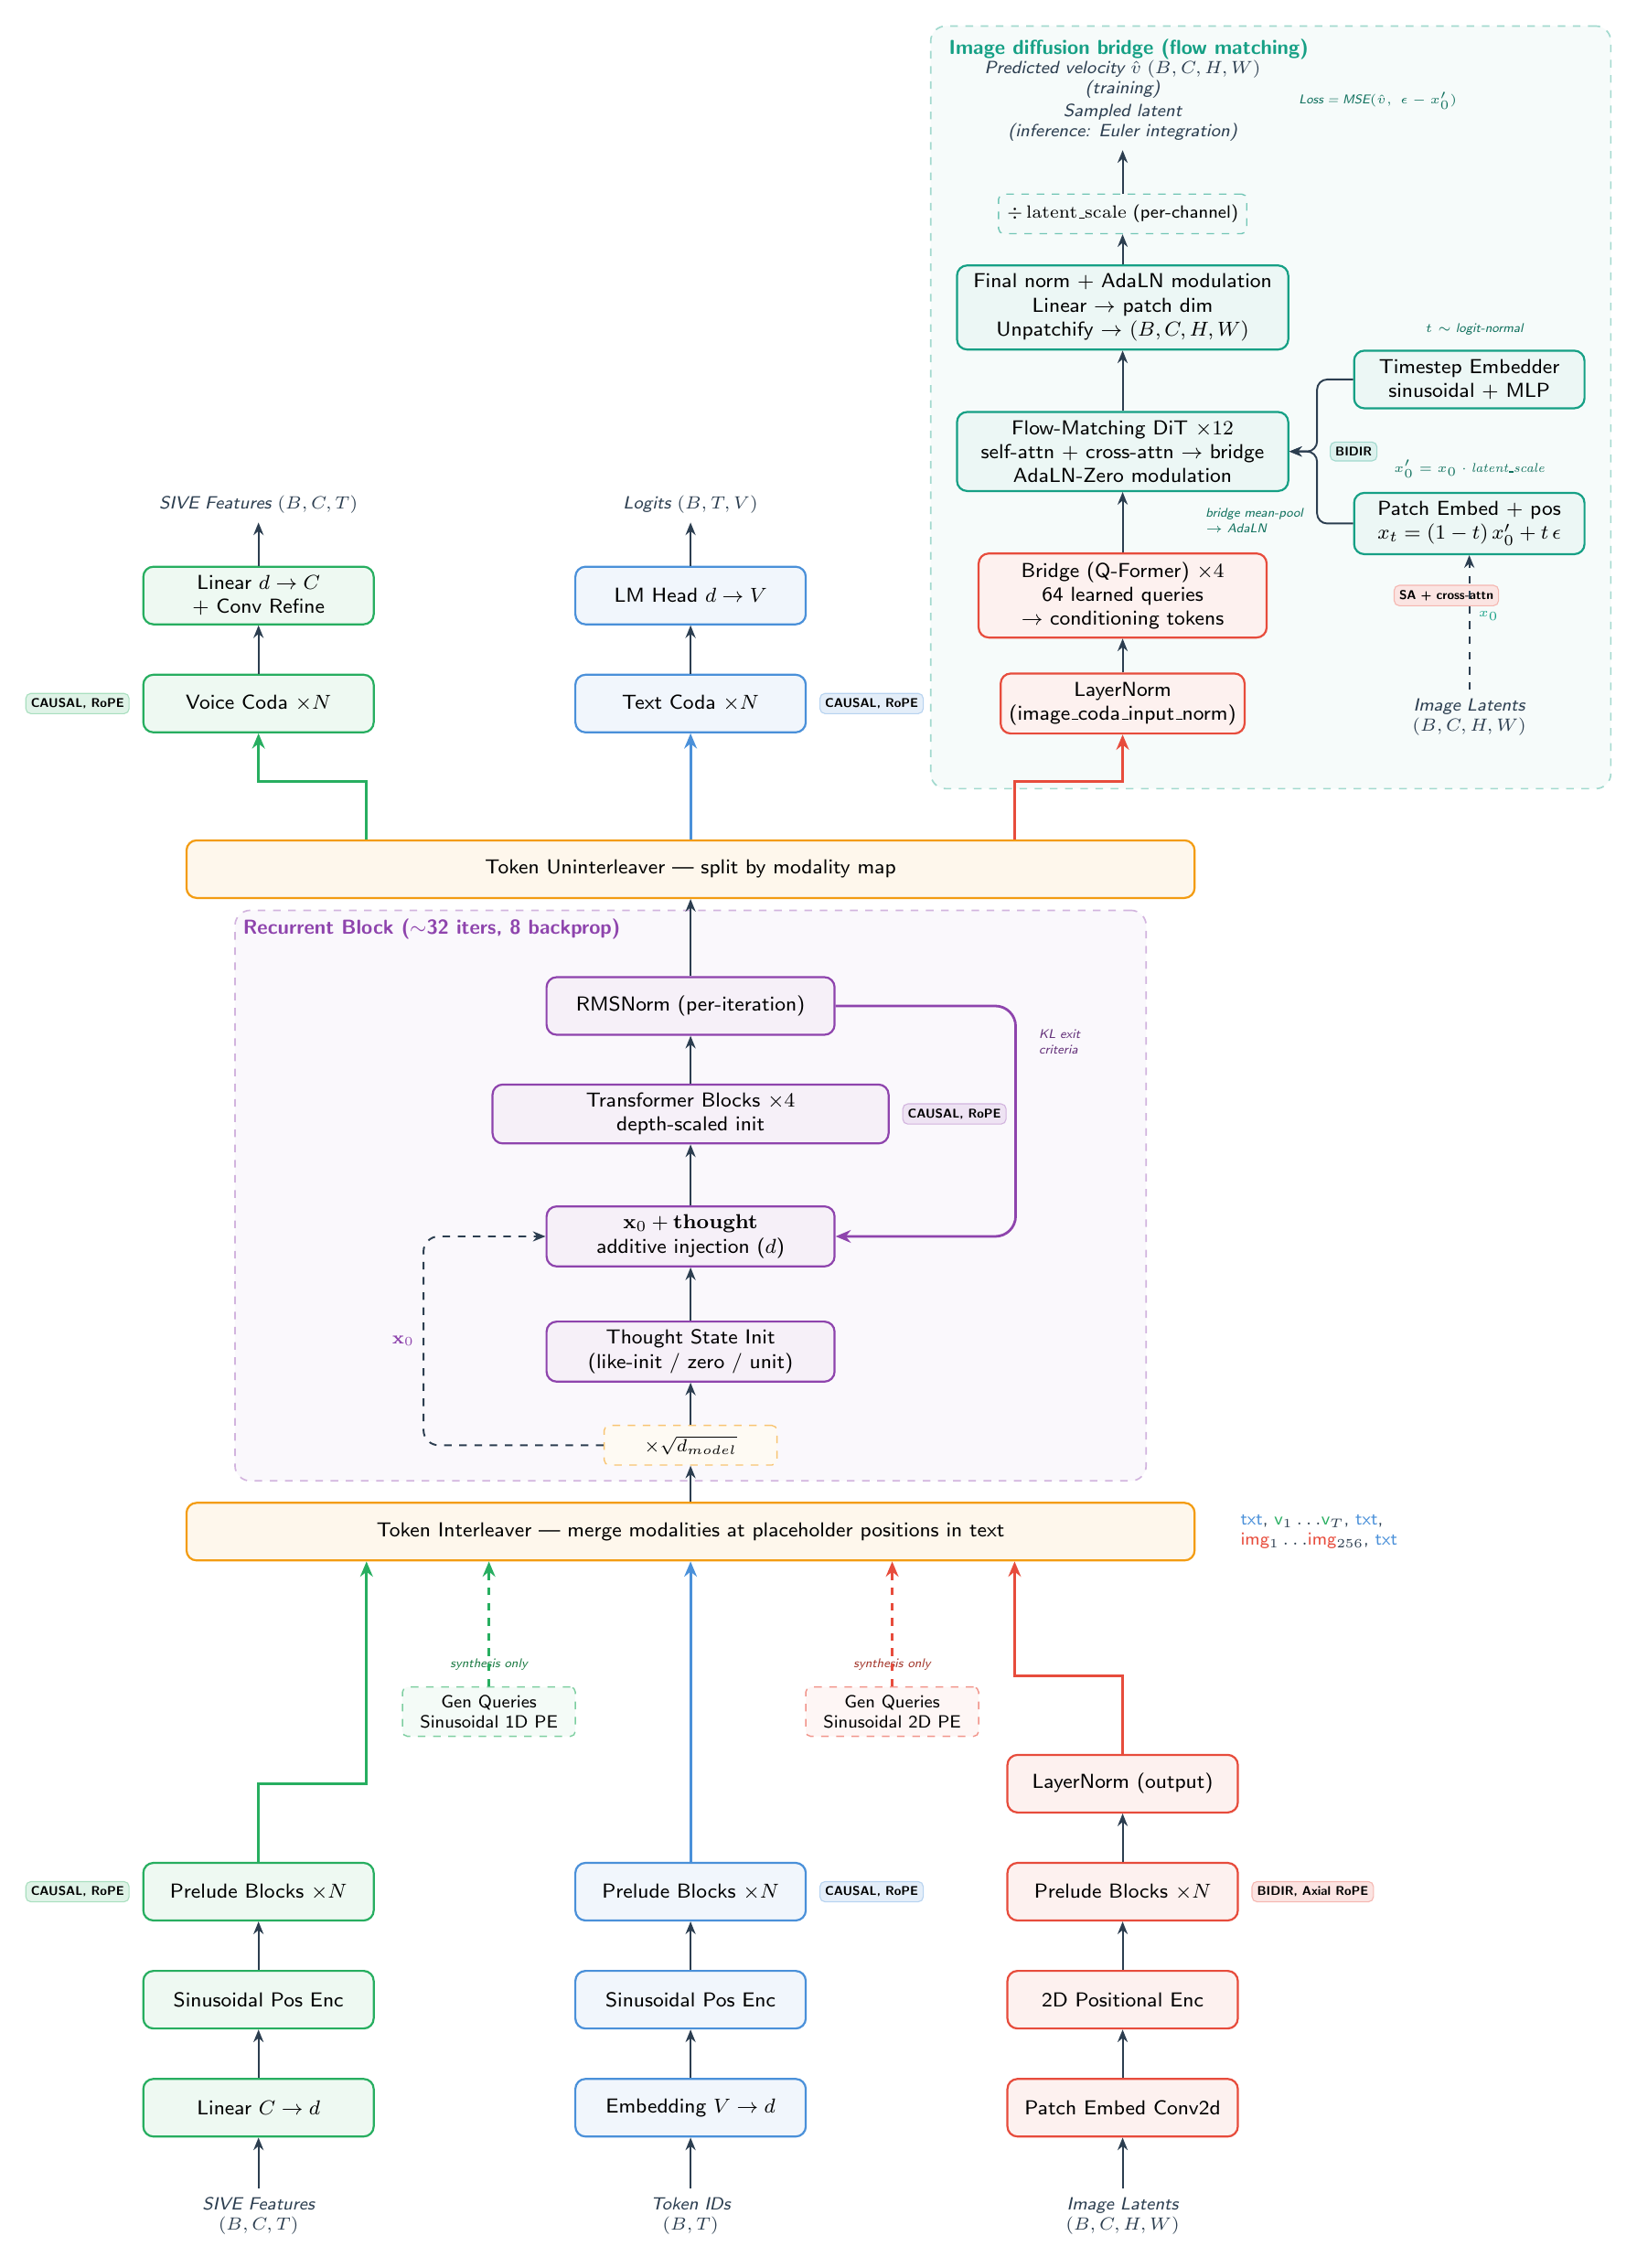
\begin{tikzpicture}

% Column X positions: voice - voiceCond - TEXT - imageCond - image - dit
\def\voiceX{0}
\def\voiceCondX{3.2}
\def\textX{6}
\def\imageCondX{8.8}
\def\imageX{12}
\def\centerX{6}

% ════════════════════════════════════════════════════════════════════
% INPUTS (row 0)
% ════════════════════════════════════════════════════════════════════
\node[iolabel] (voice_in) at (\voiceX, 0) {SIVE Features\\$(B, C, T)$};
\node[iolabel] (text_in)  at (\textX, 0)  {Token IDs\\$(B, T)$};
\node[iolabel] (image_in) at (\imageX, 0) {Image Latents\\$(B, C, H, W)$};

% ════════════════════════════════════════════════════════════════════
% FEATURE EXTRACTORS / PRELUDES
% ════════════════════════════════════════════════════════════════════

% -- Voice (left) --
\node[modbox=voicegreen] (voice_proj)    at (\voiceX, 1.5) {Linear $C \to d$};
\node[modbox=voicegreen] (voice_pos)     at (\voiceX, 3.0) {Sinusoidal Pos Enc};
\node[modbox=voicegreen] (voice_prelude) at (\voiceX, 4.5) {Prelude Blocks $\times N$};
\node[attnlabel=voicegreen, anchor=east] at ([xshift=-5pt]voice_prelude.west) {CAUSAL, RoPE};

% -- Text (center) --
\node[modbox=textblue] (text_embed)   at (\textX, 1.5) {Embedding $V \to d$};
\node[modbox=textblue] (text_pos)     at (\textX, 3.0) {Sinusoidal Pos Enc};
\node[modbox=textblue] (text_prelude) at (\textX, 4.5) {Prelude Blocks $\times N$};
\node[attnlabel=textblue, anchor=west] at ([xshift=5pt]text_prelude.east) {CAUSAL, RoPE};

% -- Image (right) --
\node[modbox=imagered] (image_patch)   at (\imageX, 1.5) {Patch Embed Conv2d};
\node[modbox=imagered] (image_pos)     at (\imageX, 3.0) {2D Positional Enc};
\node[modbox=imagered] (image_prelude) at (\imageX, 4.5) {Prelude Blocks $\times N$};
\node[attnlabel=imagered, anchor=west] at ([xshift=5pt]image_prelude.east) {BIDIR, Axial RoPE};
\node[modbox=imagered] (image_outnorm) at (\imageX, 6.0) {LayerNorm (output)};

% Prelude arrows
\draw[arrow] (voice_in) -- (voice_proj);
\draw[arrow] (voice_proj) -- (voice_pos);
\draw[arrow] (voice_pos) -- (voice_prelude);
\draw[arrow] (text_in) -- (text_embed);
\draw[arrow] (text_embed) -- (text_pos);
\draw[arrow] (text_pos) -- (text_prelude);
\draw[arrow] (image_in) -- (image_patch);
\draw[arrow] (image_patch) -- (image_pos);
\draw[arrow] (image_pos) -- (image_prelude);
\draw[arrow] (image_prelude) -- (image_outnorm);

% ════════════════════════════════════════════════════════════════════
% SYNTHESIS PATH: Gen Queries (positional_only mode --- no learned
% component, no text conditioning cross-attention)
% ════════════════════════════════════════════════════════════════════

% Voice synthesis: just sinusoidal 1D PE
\node[annobox=voicegreen] (voice_genq) at (\voiceCondX, 7.0) {Gen Queries\\Sinusoidal 1D PE};
\node[font=\tiny\sffamily\itshape, text=voicegreen!70!black, anchor=south]
  at ([yshift=3pt]voice_genq.north) {synthesis only};

% Image synthesis: just sinusoidal 2D PE
\node[annobox=imagered] (image_genq) at (\imageCondX, 7.0) {Gen Queries\\Sinusoidal 2D PE};
\node[font=\tiny\sffamily\itshape, text=imagered!70!black, anchor=south]
  at ([yshift=3pt]image_genq.north) {synthesis only};

% ════════════════════════════════════════════════════════════════════
% TOKEN INTERLEAVER
% ════════════════════════════════════════════════════════════════════

\node[widebox=interleaveamber, minimum width=14cm] (interleaver) at (\centerX, 9.5)
  {Token Interleaver --- merge modalities at placeholder positions in text};

% Embed scale
\node[annobox=interleaveamber] (scale) at (\centerX, 10.7) {$\times \sqrt{d_{model}}$};

% Arrows into interleaver — from preludes and gen queries
\draw[thickarrow=voicegreen] (voice_prelude) -- ++(0, 1.5) -| ([xshift=-4.5cm]interleaver.south);
\draw[thickdasharrow=voicegreen] (voice_genq) -- ++(0, 1.0) -| ([xshift=-2.8cm]interleaver.south);
\draw[thickarrow=textblue] (text_prelude) -- ++(0, 1.0) -| ([xshift=0cm]interleaver.south);
\draw[thickarrow=imagered] (image_outnorm) -- ++(0, 1.5) -| ([xshift=4.5cm]interleaver.south);
\draw[thickdasharrow=imagered] (image_genq) -- ++(0, 1.0) -| ([xshift=2.8cm]interleaver.south);

\draw[arrow] (interleaver) -- (scale);

% Interleaved sequence visualization
\node[font=\scriptsize\sffamily, text=darkgray, anchor=west, align=left]
  at ([xshift=0.5cm]interleaver.east)
  {{\color{textblue}txt}, {\color{voicegreen}v}$_1 \ldots${\color{voicegreen}v}$_T$,
   {\color{textblue}txt},\\
   {\color{imagered}img}$_1 \ldots${\color{imagered}img}$_{256}$,
   {\color{textblue}txt}};

% ════════════════════════════════════════════════════════════════════
% RECURRENT BLOCK (additive injection variant)
% ════════════════════════════════════════════════════════════════════

\node[modbox=recurrentpurple, minimum width=4.0cm] (thought_init) at (\centerX, 12.0)
  {Thought State Init\\(like-init / zero / unit)};

\node[modbox=recurrentpurple, minimum width=4.0cm] (combine) at (\centerX, 13.6)
  {$\mathbf{x}_0 + \mathbf{thought}$\\additive injection ($d$)};

\node[modbox=recurrentpurple, minimum width=5.5cm] (recblocks) at (\centerX, 15.3)
  {Transformer Blocks $\times 4$\\depth-scaled init};
\node[attnlabel=recurrentpurple, anchor=west] at ([xshift=5pt]recblocks.east) {CAUSAL, RoPE};

\node[modbox=recurrentpurple, minimum width=4.0cm] (postnorm) at (\centerX, 16.8)
  {RMSNorm (per-iteration)};

% Background
\coordinate (rec_right_pad) at ([xshift=3.0cm]recblocks.east);
\coordinate (rec_left_pad) at ([xshift=-3.0cm]recblocks.west);
\begin{scope}[on background layer]
  \node[groupbg=recurrentpurple, inner sep=16pt,
    fit=(scale)(postnorm)(rec_right_pad)(rec_left_pad), yshift=10pt] (recbg) {};
\end{scope}

\node[seclabel=recurrentpurple, anchor=north west] at (recbg.north west)
  {Recurrent Block (${\sim}$32 iters, 8 backprop)};

% Arrows
\draw[arrow] (scale) -- (thought_init);
\draw[arrow] (thought_init) -- (combine);
\draw[arrow] (combine) -- (recblocks);
\draw[arrow] (recblocks) -- (postnorm);

% Loop-back arrow — use node coordinates for precise alignment
\draw[thickarrow=recurrentpurple, rounded corners=8pt]
  (postnorm.east) -- ++(2.5, 0) |- (combine.east);

% x_0 injection (left side)
\draw[dasharrow, rounded corners=6pt]
  (scale.west) -- ++(-2.5, 0) |- (combine.west)
  node[pos=0.25, left, font=\scriptsize\sffamily\itshape, text=recurrentpurple] {$\mathbf{x}_0$};

% KL label on the loop-back arrow
\node[font=\tiny\sffamily\itshape, text=recurrentpurple!70!black, anchor=west, align=left]
  at ([xshift=2.7cm, yshift=-0.5cm]postnorm.east) {KL exit\\criteria};

% ════════════════════════════════════════════════════════════════════
% TOKEN UNINTERLEAVER
% ════════════════════════════════════════════════════════════════════

\node[widebox=interleaveamber, minimum width=14cm] (uninterleaver) at (\centerX, 18.7)
  {Token Uninterleaver --- split by modality map};

\draw[arrow] (postnorm) -- (uninterleaver);

% ════════════════════════════════════════════════════════════════════
% CODAS / GENERATORS
% Voice + Text codas unchanged from the direct-decoder variant.
% Image branch is now the flow-matching diffusion bridge.
% ════════════════════════════════════════════════════════════════════

% -- Voice coda (left) --
\node[modbox=voicegreen] (voice_coda) at (\voiceX, 21.0) {Voice Coda $\times N$};
\node[modbox=voicegreen] (voice_proj_out) at (\voiceX, 22.5) {Linear $d \to C$\\+ Conv Refine};
\node[attnlabel=voicegreen, anchor=east] at ([xshift=-5pt]voice_coda.west) {CAUSAL, RoPE};

% -- Text coda (center) --
\node[modbox=textblue] (text_coda) at (\textX, 21.0) {Text Coda $\times N$};
\node[modbox=textblue] (text_lmhead) at (\textX, 22.5) {LM Head $d \to V$};
\node[attnlabel=textblue, anchor=west] at ([xshift=5pt]text_coda.east) {CAUSAL, RoPE};

% -- Image: flow-matching diffusion bridge -----------------------------
% Stage 1: normalize the recurrent output at image positions
\node[modbox=imagered] (image_norm) at (\imageX, 21.0)
  {LayerNorm\\(image\_coda\_input\_norm)};

% Stage 2: bridge --- Q-Former-style cross-attention from learned queries
\node[modbox=imagered, minimum width=4cm] (image_bridge) at (\imageX, 22.5)
  {Bridge (Q-Former) $\times 4$\\64 learned queries\\$\to$ conditioning tokens};
\node[attnlabel=imagered, anchor=west] at ([xshift=1.75cm]image_bridge.east) {SA + cross-attn};

% Stage 3: DiT backbone
\node[modbox=ditteal, minimum width=4.6cm] (image_dit) at (\imageX, 24.5)
  {Flow-Matching DiT $\times 12$\\
   self-attn $+$ cross-attn $\to$ bridge\\
   AdaLN-Zero modulation};
\node[attnlabel=ditteal, anchor=west] at ([xshift=16pt]image_dit.east) {BIDIR};

% Stage 4: final layer + unpatchify
\node[modbox=ditteal, minimum width=4.6cm] (image_finallayer) at (\imageX, 26.5)
  {Final norm $+$ AdaLN modulation\\
   Linear $\to$ patch dim\\
   Unpatchify $\to$ $(B, C, H, W)$};

% Stage 5: undo latent scale
\node[annobox=ditteal] (image_unscale) at (\imageX, 27.8)
  {$\div\,\textrm{latent\_scale}$ (per-channel)};

% Side inputs to the DiT (noisy latent + timestep)
% Noise mixer: x_t = (1-t)·x_0_scaled + t·eps
\node[modbox=ditteal, minimum width=3.2cm] (image_noisemix) at ([xshift=2.5cm, yshift=-1cm]image_dit.east)
  {Patch Embed $+$ pos\\
   $x_t = (1-t)\,x_0' + t\,\epsilon$};
\node[font=\tiny\sffamily\itshape, text=ditteal!70!black, anchor=south, align=center]
  at ([yshift=2pt]image_noisemix.north)
  {$x_0' = x_0 \cdot \textrm{latent\_scale}$};

% Timestep embedder
\node[modbox=ditteal, minimum width=3.2cm] (image_tembed) at ([xshift=2.5cm, yshift=1cm]image_dit.east)
  {Timestep Embedder\\sinusoidal $+$ MLP};
\node[font=\tiny\sffamily\itshape, text=ditteal!70!black, anchor=center, align=center]
  at ([xshift=2pt, yshift=8pt]image_tembed.north)
  {$t \sim$ logit-normal};

% Bridge global pool annotation
\node[font=\tiny\sffamily\itshape, text=ditteal!70!black, anchor=west, align=left]
  at ([xshift=-28pt, yshift=4pt]image_bridge.east |- 0,23.4)
  {bridge mean-pool\\$\to$ AdaLN};

% Image output (training: predicted velocity; inference: sampled latent)
\node[iolabel, above=0.6cm of image_unscale, align=center] (image_out)
  {Predicted velocity $\hat v\;(B, C, H, W)$\\
   {\scriptsize (training)}\\[1pt]
   Sampled latent\\
   {\scriptsize (inference: Euler integration)}};

% Background frame for the diffusion-bridge group
\coordinate (dit_top) at ([yshift=0.6cm]image_unscale.north);
\coordinate (dit_bot) at ([yshift=-0.4cm]image_norm.south);
\begin{scope}[on background layer]
  \node[groupbg=ditteal, inner sep=10pt,
    fit=(image_norm)(image_bridge)(image_dit)(image_finallayer)(image_unscale)(image_noisemix)(image_tembed)(dit_top)(dit_bot)(image_out)] (ditbg) {};
\end{scope}
\node[seclabel=ditteal, anchor=north west] at ([xshift=4pt, yshift=-2pt]ditbg.north west)
  {Image diffusion bridge (flow matching)};

% Arrows from uninterleaver to codas
\draw[thickarrow=voicegreen] ([xshift=-4.5cm]uninterleaver.north) -- ++(0, 0.8) -| (voice_coda);
\draw[thickarrow=textblue]   ([xshift=0cm]uninterleaver.north) -- ++(0, 0.6) -| (text_coda);
\draw[thickarrow=imagered]   ([xshift=4.5cm]uninterleaver.north) -- ++(0, 0.8) -| (image_norm);

% Voice / text coda flow
\draw[arrow] (voice_coda) -- (voice_proj_out);
\draw[arrow] (text_coda) -- (text_lmhead);

% Image diffusion bridge flow
\draw[arrow] (image_norm) -- (image_bridge);
% Bridge → DiT cross-attention KV (right side of the bridge box up to the DiT)
\draw[arrow, rounded corners=4pt] (image_bridge) -- (image_dit);
% DiT internal stages
\draw[arrow] (image_dit) -- (image_finallayer);
\draw[arrow] (image_finallayer) -- (image_unscale);

% Side inputs to the DiT
% Patch embed of noisy latent → DiT (horizontal arrow into DiT's right side)
\draw[arrow, rounded corners=4pt] (image_noisemix.west) -- ++(-0.5, 0) |- (image_dit);
% Timestep embedder → DiT (slightly above for AdaLN modulation)
\draw[arrow, rounded corners=4pt] (image_tembed.west) -- ++(-0.5, 0) |- (image_dit);

\node[iolabel] (image_dit_in) at ([yshift=-2.25cm]image_noisemix.south) {Image Latents\\$(B, C, H, W)$};

% x_0 (clean LiteVAE latents) feeds the noise mixer — dashed because it
% reuses the same dataset latents that fed the prelude path.
\draw[dasharrow, rounded corners=6pt]
  (image_dit_in.north) -- (image_noisemix.south)
  node[pos=0.55, right, font=\tiny\sffamily\itshape, text=ditteal] {$x_0$};

% ════════════════════════════════════════════════════════════════════
% OUTPUTS
% ════════════════════════════════════════════════════════════════════

\node[iolabel, above=0.6cm of voice_proj_out] (voice_out) {SIVE Features $(B, C, T)$};
\node[iolabel, above=0.6cm of text_lmhead]    (text_out)  {Logits $(B, T, V)$};

\draw[arrow] (voice_proj_out) -- (voice_out);
\draw[arrow] (text_lmhead) -- (text_out);
\draw[arrow] (image_unscale) -- (image_out);

% Loss annotation
\node[font=\tiny\sffamily\itshape, text=ditteal!70!black, anchor=west, align=left]
  at ([xshift=8pt]image_out.east)
  {Loss = MSE$(\hat v,\;\epsilon - x_0')$};

\end{tikzpicture}
\end{document}
